\documentclass[a4paper]{article}
\usepackage{graphicx}
\usepackage[utf8]{inputenc}
\usepackage{scrextend}
\begin{document}
	\title{Kuitinseuranta dokumentaatio}
	\author{Kasper Koho}
	\renewcommand{\today}{6. syyskuuta 2015}
	\maketitle
	
	\pagebreak
	
	\section{Johdanto}
	\subsection{Tarkoitus}
	Järjestelmän tarkoitus on auttaa käyttäjiä seuraamaan kulutustaan ilman manuaalista tiedon syöttämistä.
	
	\subsection{Kuvaus}
	Käyttäjät voivat rekisteröityä, ja kirjauduttuaan sisään he voivat lisätä palveluun kuvia kuiteistaan. Kuitit koneluetaan ja siitä saatu data kategorioidaan.\newline
	Käyttäjä itse määrittelee kategoriat ja mitkä tuotteet menevät mihinkin kategoriaan.
	
	\subsection{Teknologia}
	Projekti toteutetaan projektin tekijän omalla palvelimella käyttäen PHP ja MySQL teknologioita. Käyttäjältä vaaditaan JavaScriptiä jotta sivusto toimisi oikein. Tietokantaa ei voi vaihtaa lennosta, vaan tietokantakyselyitä on muokattava.
	
	\section{Käyttötapaukset}
	\subsection{Kaavio}
	\begin{center}
		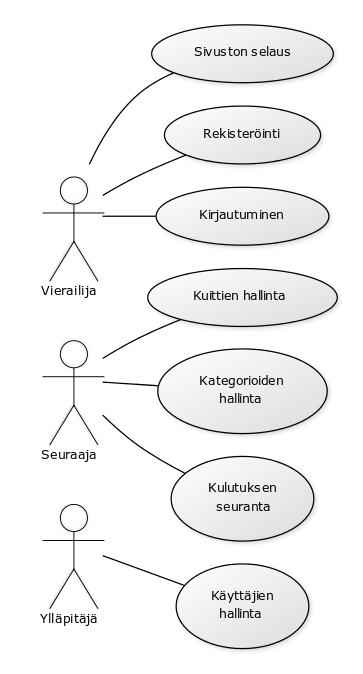
\includegraphics[scale=0.8]{kayttotapauskaavio}
	\end{center}
	
	\subsection{Käyttäjäryhmät}
	\subsubsection{Vierailija}
	Vierailijalla tarkoitetaan käyttäjää, joka ei ole kirjautunut sivustolle.
	
	\subsubsection{Seuraaja}
	Seuraajalla tarkoitetaan käyttäjää, joka on rekisteröitynyt ja kirjautunut sivustolle.
	
	\subsubsection{Ylläpitäjä}
	Ylläpitäjällä tarkoitetaan käyttäjää, joka on rekisteröitynyt ja kirjautunut sivustolle, ja jolla on ylläpitäjän oikeudet.
	
	\subsection{Käyttötapauskuvaukset}
	\subsubsection{Vierailija}
	\begin{addmargin}[2em]{0em}
		\begin{description}
			\item[Sivuston selaus] \hfill \\
				Vierailija voi selata sivuston etusivua.
			\item[Rekisteröinti] \hfill \\
				Vierailija voi rekisteröidä itselleen tunnuksen.
			\item[Kirjautuminen] \hfill \\
				Vierailija voi kirjautua sisään, mikäli hänellä on tunnus.
		\end{description}
	\end{addmargin}

	
	\subsubsection{Seuraaja}
	\begin{addmargin}[2em]{0em}
		\begin{description}
			\item[Kuittien hallinta] \hfill \\
				Seuraaja voi selata, lisätä, muuttaa ja poistaa omia kuittejaan.
			\item[Kategorioiden hallinta] \hfill \\
				Seuraaja voi selata, lisätä, muuttaa ja poistaa omia kategorioitaan.
			\item[Kulutuksen seuranta] \hfill \\
				Seuraaja voi katsella omaa kulutustaan.
		\end{description}
	\end{addmargin}
	
	\subsubsection{Ylläpitäjä}
	\begin{addmargin}[2em]{0em}
		\begin{description}
			\item[Käyttäjien hallinta] \hfill \\
				Ylläpitäjä voi selata, lisätä, muuttaa ja poistaa järjestelmän käyttäjiä.
		\end{description}
	\end{addmargin}
\end{document}